\documentclass[10pt,a4paper]{report}
\usepackage[utf8]{inputenc}
\usepackage{amsmath}
\usepackage{mathtools}
\usepackage{amsfonts}
\usepackage{amssymb}
\usepackage{graphicx}
\usepackage{hyperref}
\usepackage{bm}
\usepackage{gensymb}
\usepackage{listings}
\usepackage[left=2cm,right=2cm,top=2cm,bottom=2cm]{geometry}
\usepackage{breqn}
\setlength\parindent{0pt}
\graphicspath{{./images/}}
\newcommand{\legendre}[2]{(\frac{#1}{#2})}

\begin{document}


\textbf{CATAM Part II - 14.6 - Isolating Integrals for Geodesic Motion}
\thispagestyle{empty}

\newpage

\subsection*{Introduction}

Throughout this project I code in python, making use of the SymPy package for symbolic mathematics. We also use the GraviPy package, built on top of SymPy, giving us data structures to store and manipulate the kinds of tensors that appear in general relativity. We'll only need it to compute the Christoffel symbols. SciPy will be used to perform numerical integration. 
\subsection*{Question 1}

We use the equivalent action 

\begin{equation*}
\mathcal{S}=\int \mathcal{L} d\tau
\end{equation*}
\begin{equation*}
\mathcal{L}=g_{ij}\dot{x}^i\dot{x}^j = g_{tt}\dot{t}^2 + 2g_{t\phi}\dot{t}\dot{\phi}+g_{\phi\phi}\dot{\phi}^2+g_{rr}\dot{r}^2+g_{\theta\theta}\dot{\theta}^2
\end{equation*} 

where the dot denotes differentiation with respect to $\tau$. The conserved quantities come from the lack of dependence of $\mathcal{L}$ on $t, \phi$.\\

No $t$ dependence gives

\begin{equation}
\frac{\partial \mathcal{L}}{\partial t} = 2g_{tt}\dot{t} + 2g_{t\phi}\dot{\phi} = 2E
\label{Edef}
\end{equation}

for $E$ constant, and similarly no $\phi$ dependence gives 

\begin{equation}
\frac{\partial \mathcal{L}}{\partial \phi} = 2g_{t\phi}\dot{t}+2g_{\phi\phi}\dot{\phi} = -2L_z
\label{Ldef}
\end{equation}

for $L_z$ constant. We get a further conserved quantity from no $\tau$ dependence

\begin{equation}
\mathcal{L} - \dot{x}^i \frac{\partial \mathcal{L}}{\partial \dot{x}^i} = -\mathcal{L} = -1
\label{Qdef}
\end{equation}

where $\mathcal{L} = 1$ is by timelikeness \footnote{this is because of our signature, in the course this would be -1} \\

To determine the effective potential we sub (\ref{Edef}) and (\ref{Ldef}) into (\ref{Qdef}). (\ref{Edef}) and (\ref{Ldef}) give a system of 2 equations for $\dot{t}, \dot{\phi}$ which can be solved to give

\begin{equation}
\dot{t} = \frac{Eg_{\phi\phi}+L_zg_{t\phi}}{g_{tt}g_{\phi\phi}-g_{t\phi}^2}
\end{equation}

\begin{equation}
\dot{\phi} = -\frac{Eg_{t\phi}+L_zg_{tt}}{g_{tt}g_{\phi\phi}-g_{t\phi}^2}
\end{equation}

and thus (\ref{Qdef}) becomes (after some algebra)

\begin{equation}
g_{rr}\dot{r}^2+g_{\theta\theta}\dot{\theta}^2 = -V_{eff}(r, \theta, E, L_z)
\label{effpot}
\end{equation}
\begin{equation*}
V_{eff}(r, \theta, E, L_z) = -1 + \frac{E^2g_{\phi\phi} + L_z^2g_{tt} + 2ELg_{t\phi}}{g_{tt}g_{\phi\phi}-g_{t\phi}^2}
\end{equation*}

\subsection*{Question 2}
Computing the Christoffel symbols and returning latex is pretty straightforward using GraviPy, and was done using $compute\_kerr\_christoffel.py$. The non zero Christoffel symbols (up to symmetry) in the lower indices are displayed below. We make some attempt to simplify the expressions through substituting in $\Sigma$ and $\Delta$, but there may exist simpler forms our program had missed. This won't matter for later computation. Here's what we get:

\small\begin{align*}
\Gamma^t_{tr} = - \frac{m (a^{2} + r^{2}) (a^{2} \cos^{2}{(\theta )} - r^{2})}{\Delta \Sigma^{2}}\\
\Gamma^t_{t\theta} = - \frac{a^{2} m r \sin{(2 \theta )}}{\Sigma^{2}}\\
\Gamma^t_{r\phi} = - \frac{a m (2 \Sigma r^{2} + a^{4} \sin^{2}{(\theta )} - a^{4} + a^{2} r^{2} \sin^{2}{(\theta )} + r^{4}) \sin^{2}{(\theta )}}{\Delta \Sigma^{2}}\\
\Gamma^t_{\theta\phi} = - \frac{2 a m r (\Sigma a^{2} + \Sigma r^{2} - a^{4} + 2 a^{2} m r \sin^{2}{(\theta )} - 2 a^{2} r^{2} - r^{4}) \sin{(\theta )} \cos{(\theta )}}{\Delta \Sigma^{2}}\\
\Gamma^r_{tt} = \frac{\Delta m (- a^{2} \cos^{2}{(\theta )} + r^{2})}{\Sigma^{3}}\\
\Gamma^r_{t\phi} = \frac{\Delta a m (a^{2} \cos^{2}{(\theta )} - r^{2}) \sin^{2}{(\theta )}}{\Sigma^{3}}\\
\Gamma^r_{rr} = \frac{r}{\Sigma} + \frac{m}{\Delta} - \frac{r}{\Delta}\\
\Gamma^r_{r\theta} = - \frac{a^{2} \sin{(2 \theta )}}{2 \Sigma}\\
\Gamma^r_{\theta\theta} = - \frac{\Delta r}{\Sigma}\\
\Gamma^r_{\phi\phi} = \frac{\Delta (- 8 \Sigma^{2} r + a^{4} m (\cos{(4 \theta )} - 1) + 8 a^{2} m r^{2} \sin^{2}{(\theta )}) \sin^{2}{(\theta )}}{8 \Sigma^{3}}\\
\Gamma^\theta_{tt} = - \frac{a^{2} m r \sin{(2 \theta )}}{\Sigma^{3}}\\
\Gamma^\theta_{t\phi} = \frac{a m r (a^{2} + r^{2}) \sin{(2 \theta )}}{\Sigma^{3}}\\
\Gamma^\theta_{rr} = \frac{a^{2} \sin{(2 \theta )}}{2 \Delta \Sigma}\\
\Gamma^\theta_{r\theta} = \frac{r}{\Sigma}\\
\Gamma^\theta_{\theta\theta} = - \frac{a^{2} \sin{(2 \theta )}}{2 \Sigma}\\
\Gamma^\theta_{\phi\phi} = - \frac{(\Sigma (\Sigma a^{2} + \Sigma r^{2} + 2 a^{2} m r \sin^{2}{(\theta )}) + 2 a^{2} m r (a^{2} + r^{2}) \sin^{2}{(\theta )}) \sin{(\theta )} \cos{(\theta )}}{\Sigma^{3}}\\
\Gamma^\phi_{tr} = - \frac{a m (a^{2} \cos^{2}{(\theta )} - r^{2})}{\Delta \Sigma^{2}}\\
\Gamma^\phi_{t\theta} = - \frac{2 a m r}{\Sigma^{2} \tan{(\theta )}}\\
\Gamma^\phi_{r\phi} = \frac{\Sigma^{2} r - 2 \Sigma m r^{2} - \frac{a^{4} m (\cos{(4 \theta )} - 1)}{8} - a^{2} m r^{2} \sin^{2}{(\theta )}}{\Delta \Sigma^{2}}\\
\Gamma^\phi_{\theta\phi} = \frac{2 a^{2} m^{2} r^{2} (a^{2} + r^{2}) \sin{(\theta )} \sin{(2 \theta )} + (\Sigma - 2 m r) (\Sigma (\Sigma a^{2} + \Sigma r^{2} + 2 a^{2} m r \sin^{2}{(\theta )}) + 2 a^{2} m r (a^{2} + r^{2}) \sin^{2}{(\theta )}) \cos{(\theta )}}{\Delta \Sigma^{3} \sin{(\theta )}}\\
\end{align*}

\normalsize
\subsection*{Question 3}

Using a section of $q3\_schwarzchild.py$, just as above, we calculate the non zero Christoffel symbols, finding

\small\begin{align*}
\Gamma^t_{tr} = \frac{m}{r (- 2 m + r)}\\
\Gamma^r_{tt} = \frac{m (- 2 m + r)}{r^{3}}\\
\Gamma^r_{rr} = \frac{m}{r (2 m - r)}\\
\Gamma^r_{\theta\theta} = 2 m - r\\
\Gamma^r_{\phi\phi} = (2 m - r) \sin^{2}{(\theta )}\\
\Gamma^\theta_{r\theta} = \frac{1}{r}\\
\Gamma^\theta_{\phi\phi} = - \frac{\sin{(2 \theta )}}{2}\\
\Gamma^\phi_{r\phi} = \frac{1}{r}\\
\Gamma^\phi_{\theta\phi} = \frac{1}{\tan{(\theta )}}\\
\end{align*}

\normalsize
Now substituting $\theta=\pi/2$, $g_{\phi\phi} = -r^2$, $g_{tt}=(1-2m/r)$ and $g_{t\phi} = 0$ into (\ref{effpot}), we get, making sure to use the correct signature:

\begin{equation}
V_{eff}(r, E, L_z) = -1 + \frac{E^2}{1-2m/r} - \frac{L^2}{r^2} = g_{rr}\dot{r}^2+g_{\theta\theta}\dot{\theta}^2
\label{SCVeff}
\end{equation}

which has zeros as solutions of 

\begin{equation*}
r^3(E^2-1) + 2mr^2 -L_z^2r+2mL_z^2=0
\end{equation*}

which for $E=0.97, L_z=4, m=1$ are $\approx 3.07, 7.61, 23.16$. By graphing, our potential is positive for $7.61<r<23.16$ or $2<r<3.07$ (ignoring $r<2$ within schwarzchild radius, not physical for a timelike geodesic). Now a bound orbit in the equatorial plane must have $\dot{\theta}=0$, and so (\ref{SCVeff}) becomes

\begin{equation*}
\dot{r}^2 = -(1-2/r)V_{eff}
\end{equation*}

Only some of these solutions will be bound... TODO

\subsubsection*{3a}

Using (\ref{Edef}), (\ref{Ldef}) and (\ref{SCVeff}) we can calculate initial values for $\dot{t}, \dot{phi}$ and $\dot{\theta}$ respectively. Calling the function $compute\_one\_geodesic()$ in $q3\_schwarzchild.py$, we produce the following plots using parameters $r=15, \theta=\pi/2, \dot{r}=0, E=0.97, L=4$. Some fiddling around with the integration parameters was required to get a smooth enough curve, over a few orbits. Looking at the $\phi$ plot, we have just over 3 orbits. Calculating $E$, $L_z$, and $g_{rr}\dot{r}^2+g_{\theta\theta}\dot{\theta}^2 + V_{eff}(r, \theta, E, L_z)$ at each point we get our 3 conservation laws to high precision, assuring us the numerical integration is accurate enough for our purposes .

\begin{figure}[!ht]
\begin{minipage}[b]{0.5\linewidth}
\centering
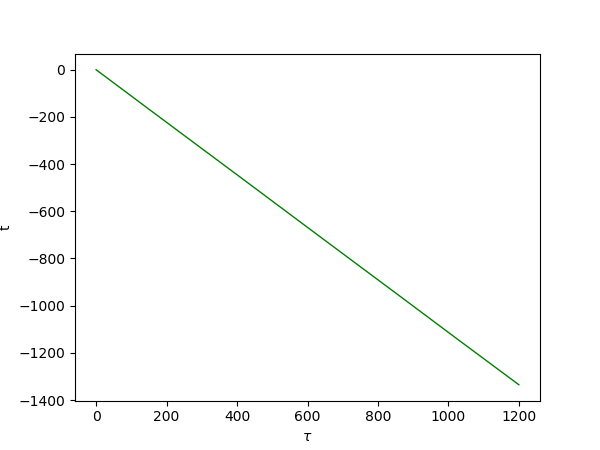
\includegraphics[width=\textwidth]{3a/t.png}
\caption{$t$}
\label{fig:figure1}
\end{minipage}
\hspace{0.5cm}
\begin{minipage}[b]{0.5\linewidth}
\centering
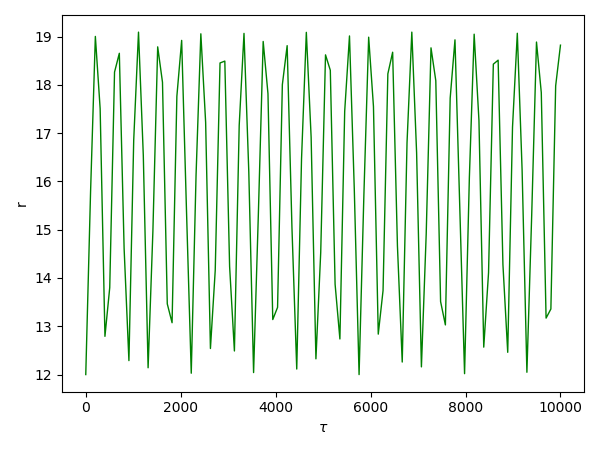
\includegraphics[width=\textwidth]{3a/r.png}
\caption{$r$}
\label{fig:figure2}
\end{minipage}
\end{figure}

\begin{figure}[!ht]
\begin{minipage}[b]{0.5\linewidth}
\centering
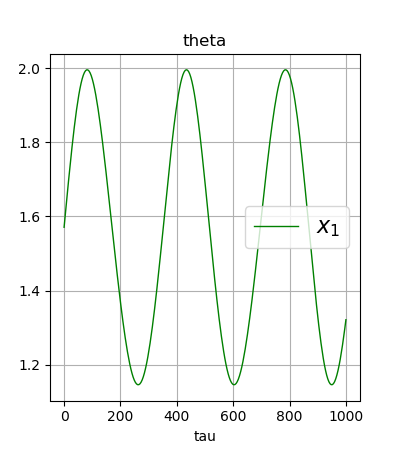
\includegraphics[width=\textwidth, height=6.5cm]{3a/theta.png}
\caption{$\theta$}
\label{fig:figure1}
\end{minipage}
\hspace{0.5cm}
\begin{minipage}[b]{0.5\linewidth}
\centering
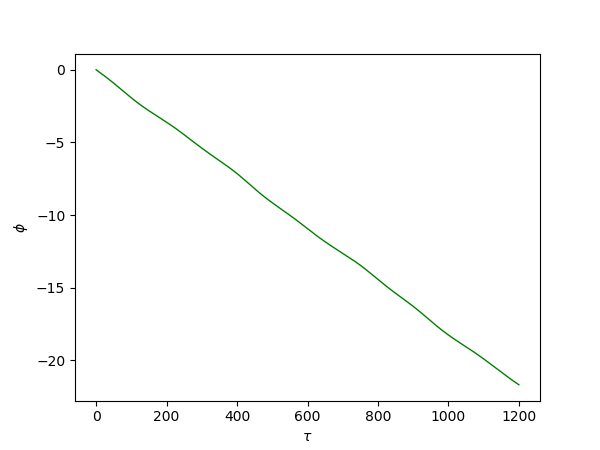
\includegraphics[width=\textwidth]{3a/phi.png}
\caption{$\phi$}
\label{fig:figure2}
\end{minipage}
\end{figure}

\begin{figure}[!ht]
\begin{minipage}[b]{0.5\linewidth}
\centering
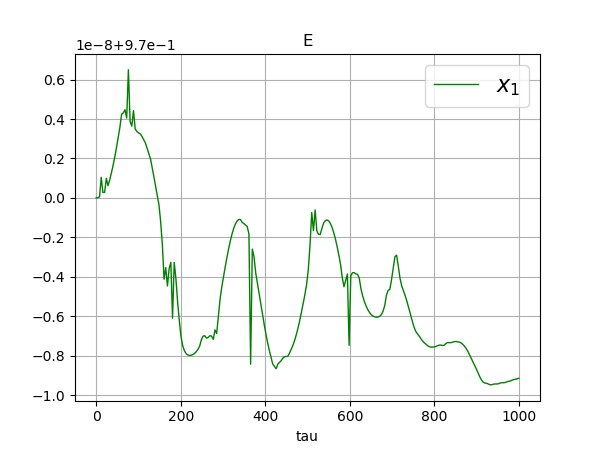
\includegraphics[width=\textwidth]{3a/E.png}
\caption{$E$}
\label{fig:figure1}
\end{minipage}
\hspace{0.5cm}
\begin{minipage}[b]{0.5\linewidth}
\centering
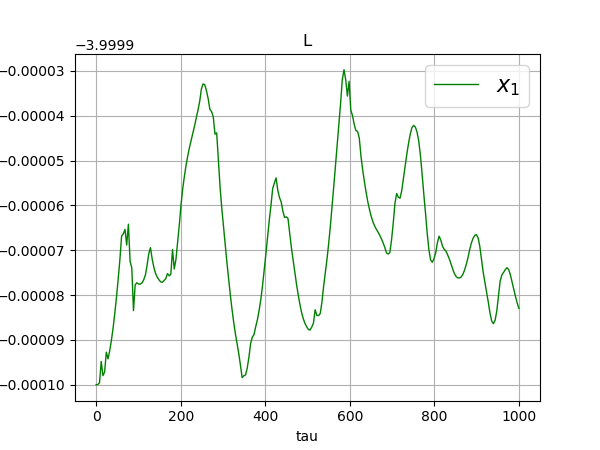
\includegraphics[width=\textwidth]{3a/L.png}
\caption{$L$}
\label{fig:figure2}
\end{minipage}
\end{figure}

\begin{figure}[!ht]
\begin{minipage}[b]{0.5\linewidth}
\centering
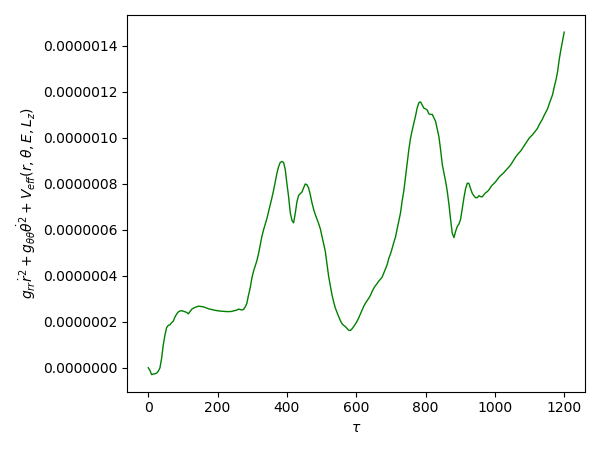
\includegraphics[width=\textwidth]{3a/Veff.png}
\caption{$g_{rr}\dot{r}^2+g_{\theta\theta}\dot{\theta}^2 + V_{eff}(r, \theta, E, L_z)$}
\label{fig:figure1}
\end{minipage}
\end{figure}

\newpage

\subsubsection*{3b}

We find as expected our code runs into issues if r is not in the range defined previously. Running the code listed under 3b in $q3.py$ with several r0 values  we obtain for fixed $\theta=\pi/2, \dot{r}=0, E=0.97, L=4$ tje following plots. We see the values form a closed curve under these conditions, with the shape of curve depending on the initial parameters

\begin{figure}[!ht]
\begin{minipage}[b]{0.5\linewidth}
\centering
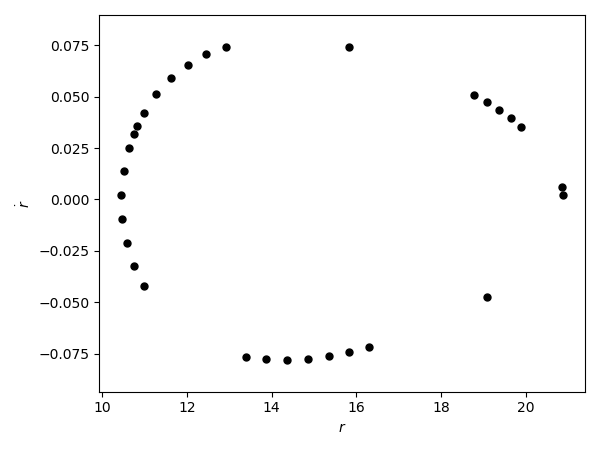
\includegraphics[width=\textwidth]{3b/r0=10,E=0.97,L=4.png}
\caption{$r_0=10$}
\label{fig:figure1}
\end{minipage}
\hspace{0.5cm}
\begin{minipage}[b]{0.5\linewidth}
\centering
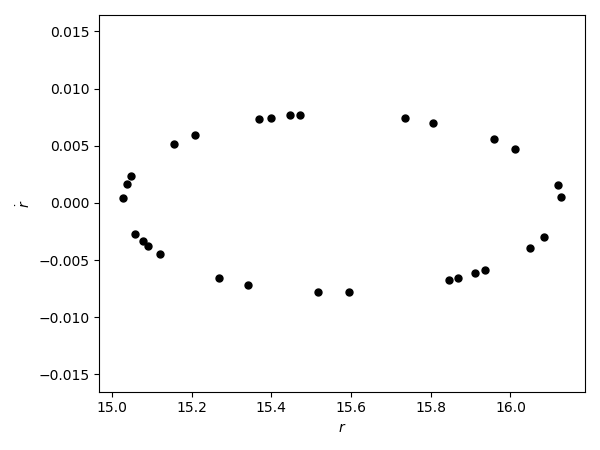
\includegraphics[width=\textwidth]{3b/r0=15,E=0.97,L=4.png}
\caption{$r_0=15$}
\label{fig:figure2}
\end{minipage}
\end{figure}

\begin{figure}[!ht]
\begin{minipage}[b]{0.5\linewidth}
\centering
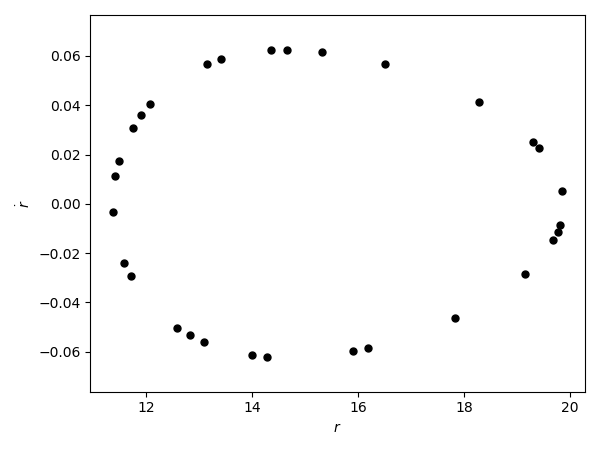
\includegraphics[width=\textwidth]{3b/r0=20,E=0.97,L=4.png}
\caption{$r_0=20$}
\label{fig:figure1}
\end{minipage}
\end{figure}



\newpage

\subsection*{Question 4}

Plotting the potential using $q4.py$ and using a numerical root finder, we see positive potential for $4.513<r<14.564$. Now modifying $q3.py$ to accomodate the Kerr metric, we produce the following Poincare maps, which all look very much like the Schwartzchild ones

\begin{figure}[!ht]
\begin{minipage}[b]{0.5\linewidth}
\centering
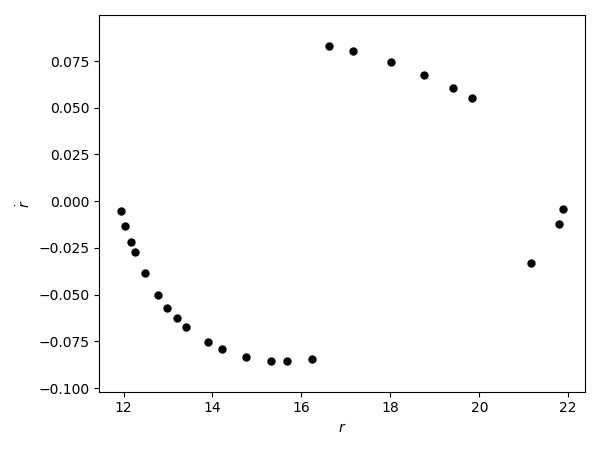
\includegraphics[width=\textwidth]{4/r0=8.png}
\caption{$r_0=10$}
\label{fig:figure1}
\end{minipage}
\hspace{0.5cm}
\begin{minipage}[b]{0.5\linewidth}
\centering
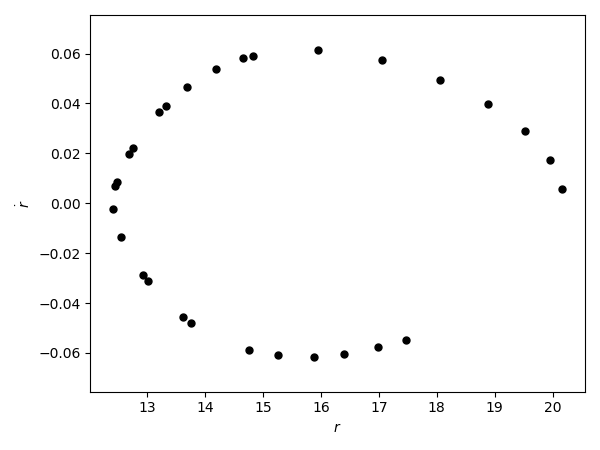
\includegraphics[width=\textwidth]{4/r0=10.png}
\caption{$r_0=15$}
\label{fig:figure2}
\end{minipage}
\end{figure}

\begin{figure}[!ht]
\begin{minipage}[b]{0.5\linewidth}
\centering
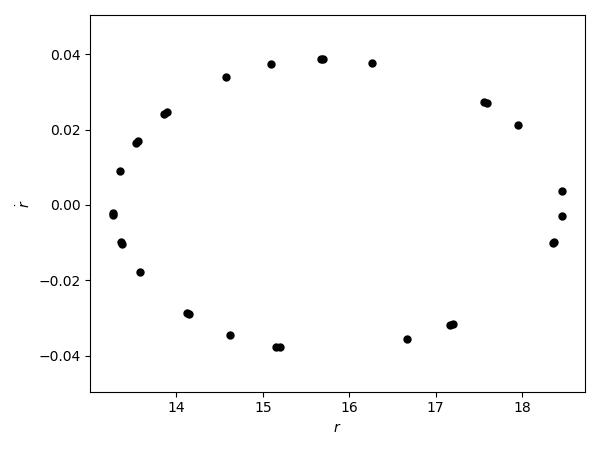
\includegraphics[width=\textwidth]{4/r0=12.png}
\caption{$r_0=20$}
\label{fig:figure1}
\end{minipage}
\end{figure}




\subsection*{Question 5}
The script $q5.py$ attempts to symbolically simplify a hand computed expression for $\dot{Q}$ by symbolically calculating and substituting in $\ddot{\theta}$ in terms of $r,m,a,\dot{theta}, \dot{t}, \dot{r}$ and $\dot{\phi}$ from the geodesic equation and Christoffel symbols. I couldn't manage to get this to work.\\

In the $a=0$ limit Q becomes

\begin{equation*}
Q = L_z^2\csc^2{\theta} + r^2\dot{\theta}^2
\end{equation*}

choosing $\theta(\tau) = \pi/2$, which we are always free to do, we get 

\begin{equation*}
Q = L_z^2
\end{equation*}

the square of the total orbital angular momentum.
\tiny
\begin{align*}
- \frac{2 \left(- \Delta \Sigma^{2} \dot{\phi}^{2} a^{2} - \Delta \Sigma^{2} \dot{\phi}^{2} r^{2} + \Delta \Sigma^{2} \dot{\theta}^{2} a^{2} + \Delta \Sigma \delta a^{2} + \Delta \Sigma \dot{\phi}^{2} a^{4} - 2 \Delta \Sigma \dot{\phi}^{2} a^{2} m r \sin^{2}{\left(\theta \right)} + 2 \Delta \Sigma \dot{\phi}^{2} a^{2} r^{2} + \Delta \Sigma \dot{\phi}^{2} r^{4} - \Delta \Sigma \dot{t}^{2} a^{2} + 2 \Delta \dot{\phi}^{2} a^{4} m r \sin^{2}{\left(\theta \right)} + 2 \Delta \dot{\phi}^{2} a^{2} m r^{3} \sin^{2}{\left(\theta \right)} - 4 \Delta \dot{\phi} \dot{t} a^{3} m r \sin^{2}{\left(\theta \right)} + 2 \Delta \dot{t}^{2} a^{2} m r + \Sigma^{2} \dot{r}^{2} a^{2}\right) \sin{\left(\theta \right)} \cos{\left(\theta \right)}}{\Delta \Sigma}
\end{align*}


\end{document}


